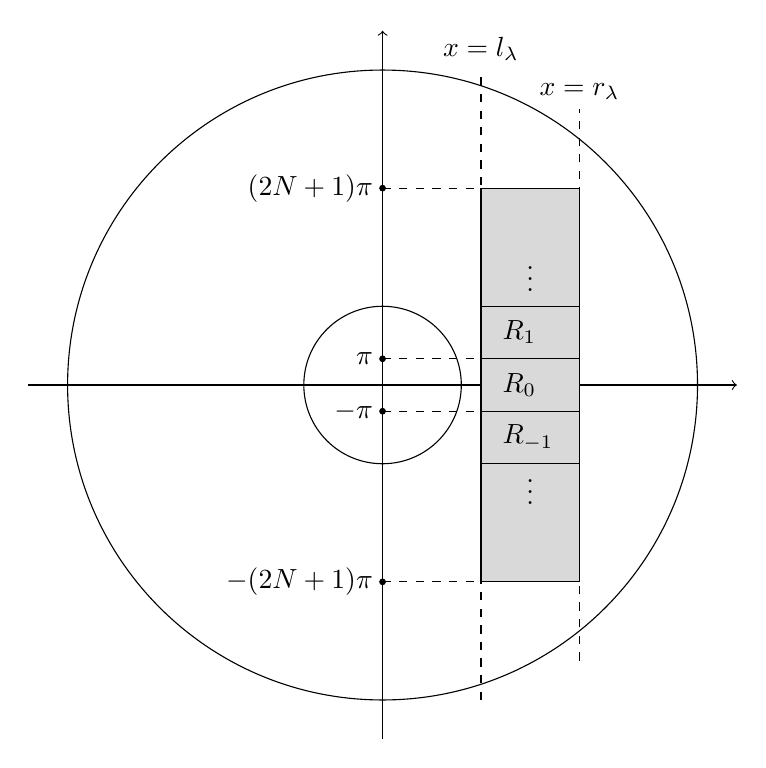
\begin{tikzpicture}
\definecolor{siva}{gray}{0.75}

\draw[->] (-4.5, 0) -- (4.5, 0);
\draw[->] (0, -4.5) -- (0, 4.5);

\draw (0, 0) circle (1);
\draw (0, 0) circle (4);

\draw[dashed] (1.25, -4) -- (1.25, 4)
node[anchor=south] {$x = l_\lambda$};
\draw[dashed] (2.5, -3.5) -- (2.5, 3.5)
node[anchor=south] {$x = r_\lambda$};

\draw[fill=gray!30] (1.25, -2.5) rectangle (2.5, 2.5);

\draw[dashed] (0, 2.5) -- (1.25, 2.5);
\draw[dashed] (0, 0.333) -- (1.25, 0.333);
\draw[dashed] (0, -0.333) -- (1.25, -0.333);
\draw[dashed] (0, -2.5) -- (1.25, -2.5);

\draw (1.25, 2.5) -- (2.5, 2.5);
\draw (1.25, 1) -- (2.5, 1);
\draw (1.25, 0.333) -- (2.5, 0.333);
% \draw[dashed] (1.25, 0) -- (2.5, 0);
\draw (1.25, -0.333) -- (2.5, -0.333);
\draw (1.25, -1) -- (2.5, -1);
\draw (1.25, -2.5) -- (2.5, -2.5);

\filldraw[black] (0, 2.5) circle (1pt)
    node[left]  {$(2N + 1) \pi$};
\filldraw[black] (0, 0.333) circle (1pt)
    node[left]  {$\pi$};
\filldraw[black] (0, -0.333) circle (1pt)
    node[left]  {$-\pi$};
\filldraw[black] (0, -2.5) circle (1pt)
    node[left]  {$-(2N + 1) \pi$};

% \draw[->] (4, 2) -- (2, 0.7);
% \draw[->] (4, 1) -- (2, 0.2);
% \draw[->] (4, -1) -- (2, -0.7);

\node[anchor=west] at (1.4, 0.67) {$R_1$};
\node[anchor=west] at (1.4, 0) {$R_0$};
\node[anchor=west] at (1.4, -0.67) {$R_{-1}$};
\node[anchor=center] at (1.875, -1.25) {$\vdots$};
\node[anchor=center] at (1.875, 1.45) {$\vdots$};

\end{tikzpicture}